\documentclass[tikz]{standalone}
\usepackage{bm}
\usepackage{stix}

\def \layersep {2 cm}
\def \sitesep {0.5 cm}
\def \layerwidth {5}
\def \hiddenlayers {3}

\def \centerx {\the\numexpr \layerwidth / 2 \relax}

\newcommand{\condeq}[4]{\ifnum#1=#2#3\else#4\fi}
\newcommand{\condlt}[4]{\ifnum#1<#2#3\else#4\fi}
\newcommand{\condgt}[4]{\ifnum#1>#2#3\else#4\fi}
\newcommand{\condle}[4]{\condgt{#1}{#2}{#4}{#3}}
\newcommand{\condge}[4]{\condlt{#1}{#2}{#4}{#3}}

\tikzstyle{neuron}=[circle, draw]
\tikzstyle{annot}=[node distance=0.5 cm]

\begin{document}
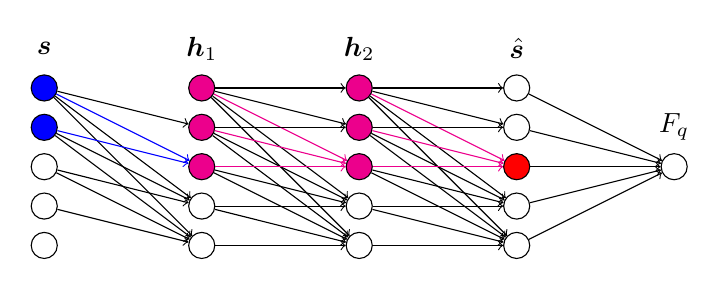
\begin{tikzpicture}[->]

\foreach \x in {1, ..., \layerwidth}
    \node[neuron, fill=\condlt{\x}{\centerx}{blue}{white}] (I\x) at (0, -\x * \sitesep) {};

\foreach \l in {1, ..., \hiddenlayers}
    \foreach \x in {1, ..., \layerwidth}
        \node[neuron, fill=\condeq{\l}{\hiddenlayers}{\condeq{\x}{\centerx}{red}{white}}{\condle{\x}{\centerx}{magenta}{white}}] (H\l\x) at (\layersep * \l, -\x * \sitesep) {};

\node[neuron] (F) at ({\layersep * (\hiddenlayers + 1)}, {-(\layerwidth + 1) / 2 * \sitesep}) {};

\foreach \x in {1, ..., \the\numexpr \layerwidth - 1 \relax}
    \foreach \y in {\the\numexpr \x + 1 \relax, ..., \layerwidth}
        \draw[\condlt{\x}{\centerx}{\condeq{\y}{\centerx}{blue}{black}}{black}] (I\x) -- (H1\y);

\foreach \l in {1, ..., \the\numexpr \hiddenlayers - 1 \relax}
    \foreach \x in {1, ..., \layerwidth}
        \foreach \y in {\x, ..., \layerwidth}
            \draw[\condle{\x}{\centerx}{\condeq{\y}{\centerx}{magenta}{black}}{black}] (H\l\x) -- (H\the\numexpr \l + 1 \relax\y);

\foreach \x in {1, ..., \layerwidth}
    \draw (H\hiddenlayers\x) -- (F);

\node[annot, above of=I1] {$\bm{s}$};
\foreach \l in {1, ..., \hiddenlayers}
    \node[annot, above of=H\l1] {\condeq{\l}{\hiddenlayers}{$\hat{\bm{s}}$}{$\bm{h}_\l$}};
\node[annot, above of=F] {$F_q$};

\end{tikzpicture}
\end{document}
